\documentclass[aspectratio=169,9pt]{beamer}

\usetheme{Madrid}
\usecolortheme{seahorse}
\usepackage[utf8]{inputenc}
\usepackage{amsmath}
\usepackage{listings}
\usepackage{xcolor}
\usepackage{graphicx}
\usepackage{booktabs}
\usepackage{tabularx}

\lstdefinestyle{cli}{
  basicstyle=\ttfamily\scriptsize,
  backgroundcolor=\color{black!5},
  frame=single,
  breaklines=true,
  columns=fullflexible,
  keywordstyle=\color{blue},
}
\lstnewenvironment{cli}{\lstset{style=cli}}{}

\title{A Real 4x4 Memristor Crossbar}
\subtitle{Scaling the 2x2 crossbar to 16 real crosspoints -- layout, a real xschem schematic, and LVS}
\author{}
\date{}

\begin{document}

\frame{\titlepage}

% ---------------------------------------------------------------
\begin{frame}{What gets built, and why it's a separate, real deck}
\footnotesize
\begin{itemize}
  \item A direct, real scale-up of \texttt{crossbar2x2\_tio2\_au}
        (see the separate \texttt{crossbar2x2.tex} deck) to 4 real
        bottom-electrode rows and 4 real top-electrode columns -- 16
        real crosspoints instead of 4, same real geometry rule reused
        (1um traces, 4um row/column pitch), same real materials
        (\texttt{be\_au}/\texttt{mem\_tio2}/\texttt{te\_au}).
  \item One genuinely new real deliverable this deck adds that the
        2x2 deck never built: a real, hand-authored \textbf{xschem
        schematic} of the crossbar's own topology, batch-netlisted
        with real xschem itself to confirm its connectivity before
        trusting it for anything -- not a hand-wave circuit diagram.
  \item Kept as its own, separate document (not folded into the 2x2
        deck) because the real, found extraction limitation
        \emph{changes shape} at this scale -- worth documenting on its
        own real terms, not just restating the 2x2 finding bigger.
\end{itemize}
\end{frame}

% ---------------------------------------------------------------
\begin{frame}[fragile]{Step 1 -- the real, scaled-up topology}
Same real construction rule as the 2x2 array, carried through
literally: each row/column is a 1um-wide real trace on a real 4um
pitch, so the total real footprint is $4N+1$ microns square for $N$
rows/columns -- $9\times9$ at $N{=}2$, $17\times17$ at $N{=}4$:
\begin{center}
\begin{tabularx}{\textwidth}{lX}
\toprule
Element & Real geometry (microns) \\
\midrule
BE1..BE4 (rows) & $y \in [2,3],[6,7],[10,11],[14,15]$, each $x \in [0,17]$ \\
TE1..TE4 (columns) & $x \in [2,3],[6,7],[10,11],[14,15]$, each $y \in [0,17]$ \\
Crosspoints & \texttt{mem\_tio2}, 1x1um, at all 16 real row/column overlaps \\
Total footprint & $17\times17$um -- exact, confirmed on real GDS export (Step 5) \\
\bottomrule
\end{tabularx}
\end{center}
Same real spacings as the 2x2 array (well above the real
\texttt{BE.W.1}/\texttt{MEM1.W.1}/\texttt{MEM2.W.1}/\texttt{TE.S.1}
DRC minimums) -- DRC-safe by construction, confirmed clean in Step 5.
\end{frame}

% ---------------------------------------------------------------
\begin{frame}[fragile]{Step 2 -- a real, hand-authored Magic layout}
Same real \texttt{.mag} format as every other cell, four real rows and
four real columns instead of two:
\begin{cli}
<< be_au >>
rect 0 2 17 3
rect 0 6 17 7
rect 0 10 17 11
rect 0 14 17 15
<< te_au >>
rect 2 0 3 17
rect 6 0 7 17
rect 10 0 11 17
rect 14 0 15 17
<< mem_tio2 >>
rect 2 2 3 3      $\ldots$ -- same real pattern at all 16 real
                    row/column overlaps (omitted here for space,
                    all 16 present in the real, tracked file)
\end{cli}
\footnotesize
Same real, already-calibrated scale as the 2x2 layout (1 raw unit = 1
real micron for this tech) -- no re-calibration needed.
\end{frame}

% ---------------------------------------------------------------
\begin{frame}{Step 2, continued -- the real, live Magic window}
\begin{center}
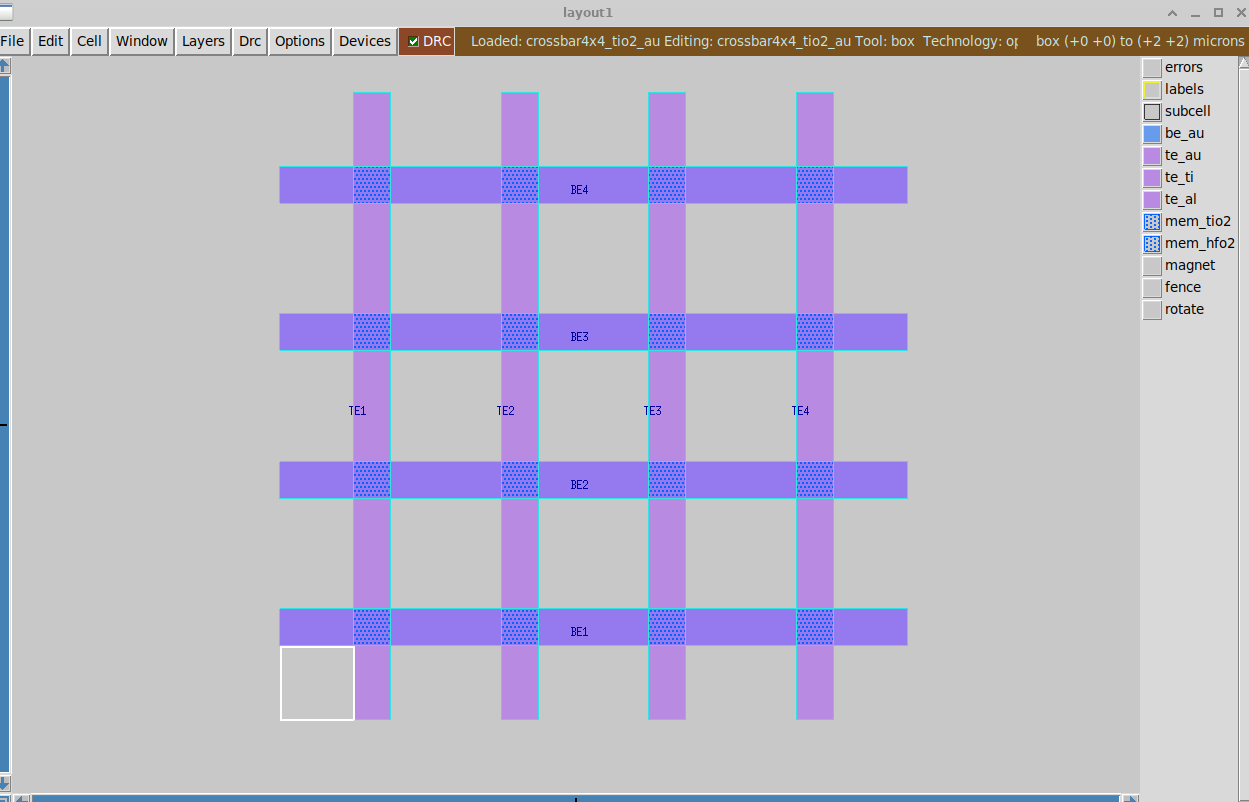
\includegraphics[width=0.6\textwidth]{figures/crossbar4x4_magic_layout.png}
\end{center}
\footnotesize
Real, live Magic, \texttt{crossbar4x4\_tio2\_au} loaded -- 4 real
\texttt{be\_au} rows crossing 4 real \texttt{te\_au} columns,
\texttt{mem\_tio2} visible at all 16 real crosspoints.
\end{frame}

% ---------------------------------------------------------------
\begin{frame}[fragile]{Step 3 -- a real LEF macro}
A new \texttt{crossbar4x4\_tio2\_au} macro, appended to the same real
combined LEF file the 2x2 macro already lives in:
\begin{center}
\begin{tabularx}{\textwidth}{lX}
\toprule
LEF field & Real value \\
\midrule
\texttt{SIZE} & 17.0 BY 17.0 (matches the real drawn footprint exactly) \\
\texttt{SYMMETRY} & X Y \\
Pins & \texttt{BE1..BE4}/\texttt{TE1..TE4}, each \texttt{DIRECTION
        INOUT}, \texttt{PORT} rect matching that row/column's own real
        position \\
\bottomrule
\end{tabularx}
\end{center}
\footnotesize
Real, live-verified: this project's own LEF parser reads the new macro
back correctly, all 8 real pins in the correct real order.
\end{frame}

% ---------------------------------------------------------------
\begin{frame}{Step 4 -- the real Library Manager}
\begin{center}
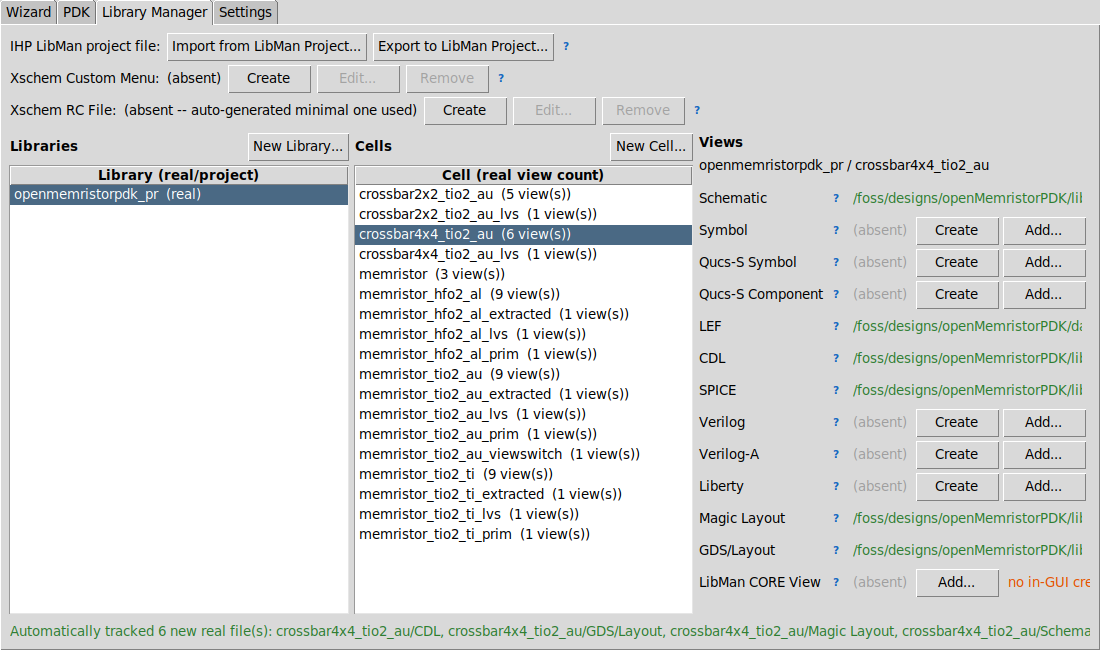
\includegraphics[width=0.65\textwidth]{figures/crossbar4x4_library_manager.png}
\end{center}
\footnotesize
Real, live: the new cell, auto-discovered under
\texttt{openmemristorpdk\_pr} from its own real files (same stem,
\texttt{crossbar4x4\_tio2\_au}) -- real CDL/SPICE/Magic
Layout/Schematic/GDS views all present.
\end{frame}

% ---------------------------------------------------------------
\begin{frame}{Step 5 -- real, live DRC}
\textbf{Run DRC} on the real Magic Layout view -- real GDS export,
then a real, live KLayout batch run against this project's own real
DRC deck, same as Step 5 of the 2x2 deck:
\begin{center}
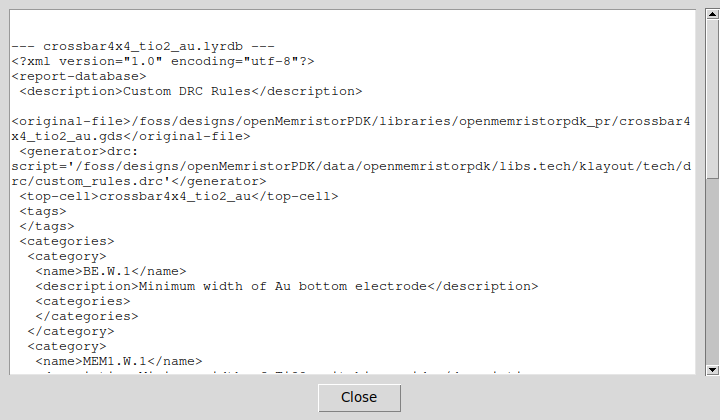
\includegraphics[width=0.65\textwidth]{figures/crossbar4x4_drc_result.png}
\end{center}
\footnotesize
Real, live result: \textbf{0 violations} -- the real 4um pitch scales
up cleanly, no new real spacing issues introduced by the extra rows
and columns.
\end{frame}

% ---------------------------------------------------------------
\begin{frame}[fragile]{Step 6 -- a real, hand-authored xschem schematic}
A genuinely new real deliverable for this deck: 16 real instances of
this project's own real \texttt{memristor\_tio2\_au} symbol, wired
into 4 real BE (row) buses and 4 real TE (column) buses. Naive,
single continuous bus wires would falsely short every row to every
column wherever they cross on the canvas -- avoided by routing each
device's own real pin to its bus through a short real stub, offset
off the neighboring pin's own real coordinate, so unrelated bus
crossings stay real, unconnected X-crossings, not accidental
T-junctions:
\begin{cli}
N -40 -60 1160 -60 {lab=BE1}
N -40 0 -40 -60 {lab=BE1}
C {iopin.sym} -160 -60 0 0 {name=pBE1 lab=BE1}
C {.../memristor_tio2_au.sym} 0 0 0 0 {name=n1 model=mm view=extracted}
\end{cli}
\footnotesize
Not trusted by inspection alone: batch-netlisted with real, live
xschem (\texttt{xschem -n -s -q}) and checked in
\texttt{tests/test\_crossbar4x4.py} -- exactly 16 real devices, every
real BE/TE row-column pair present exactly once, confirming a true
crossbar topology, not 4 accidentally-merged or accidentally-open nets.
\end{frame}

% ---------------------------------------------------------------
\begin{frame}{Step 6, continued -- the real, live xschem window}
\begin{center}
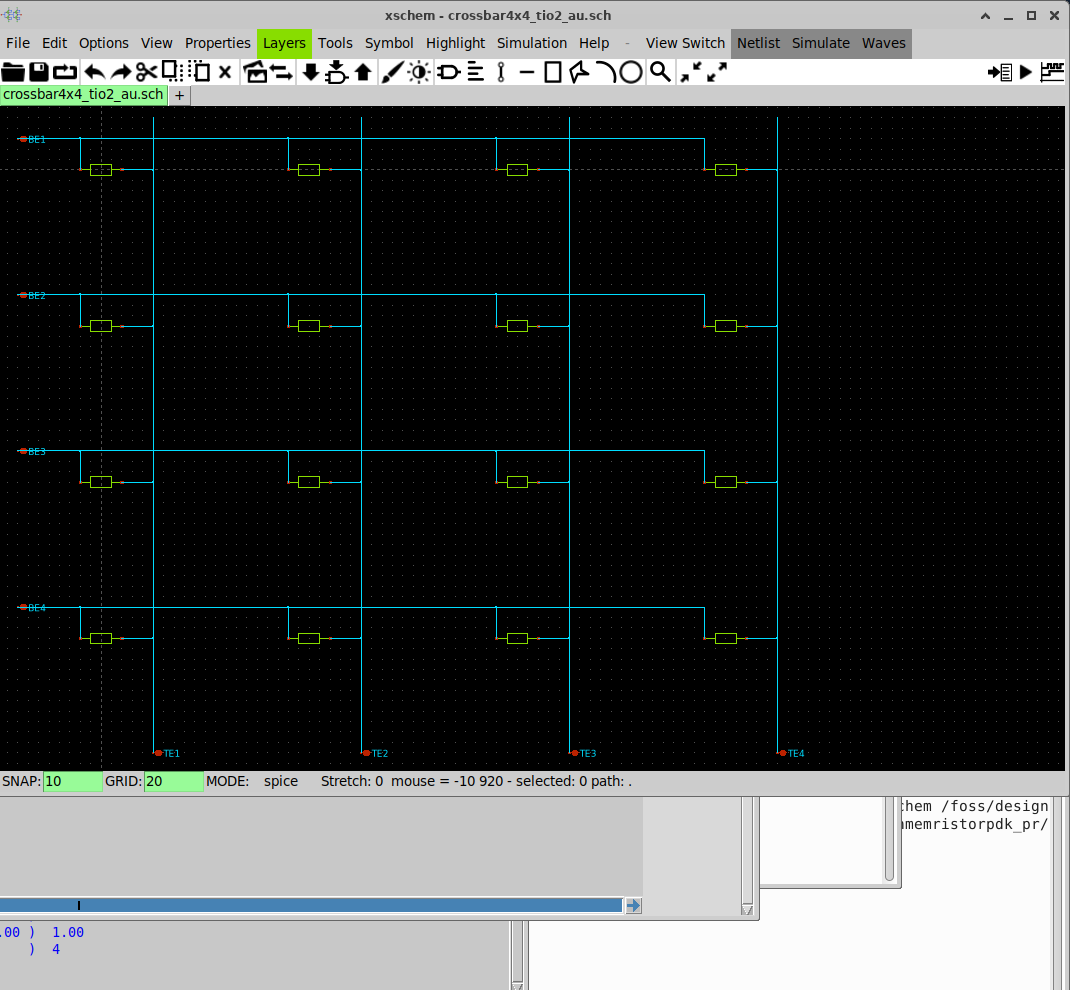
\includegraphics[width=0.6\textwidth]{figures/crossbar4x4_xschem_schematic.png}
\end{center}
\footnotesize
Real, live xschem, \texttt{crossbar4x4\_tio2\_au.sch} loaded -- the 16
real memristor symbols, the 4 real BE row buses, the 4 real TE column
buses, and the 8 real \texttt{iopin} ports.
\end{frame}

% ---------------------------------------------------------------
\begin{frame}[fragile]{Step 7 -- real extraction: the limitation gets worse, not just bigger}
\textbf{Extract to SPICE} against the real layout -- the same real
Magic device-recognition limitation found for the 2x2 array
(Step 6/6-continued of \texttt{crossbar2x2.tex}), now at 4x4 scale:
\begin{cli}
.subckt crossbar4x4_tio2_au BE1 BE2 BE3 BE4 TE1 TE2 TE3 TE4
X0 BE2 TE4 memristor_tio2_au_prim
X1 BE4 tm_14_15# memristor_tio2_au_prim
X2 BE1 tm_14_3# memristor_tio2_au_prim
X3 BE3 tm_14_11# memristor_tio2_au_prim
.ends
\end{cli}
\footnotesize
Only \textbf{4} of the real 16 crosspoints -- one per real row, the
same real "last-processed net wins" pattern as the 2x2 case, but the
real \emph{fraction} recognized drops from 2x2's 50\% (2 of 4) to 4x4's
\textbf{25\%} (4 of 16). Consistent with the real, confirmed root
cause (Magic's own core device-recognition model, not this project's
layout or \texttt{ext2spice} flags -- see the 2x2 deck's own Step 6,
continued for the real, tried-and-refuted hierarchical-extraction
fix): each real net only ever yields one real recognized device
regardless of how many real crosspoints actually sit on it, so the
real recognized fraction is $1/N$ for an $N{\times}N$ array, not a
fixed count.
\end{frame}

% ---------------------------------------------------------------
\begin{frame}[fragile]{Step 8 -- a real, hand-authored reference netlist}
Same real convention as the 2x2 deck's own Step 7 -- a real,
independent reference describing the actually-intended topology,
16 real devices this time:
\begin{cli}
.SUBCKT crossbar4x4_tio2_au BE1 BE2 BE3 BE4 TE1 TE2 TE3 TE4
*.PININFO BE1:B BE2:B BE3:B BE4:B TE1:B TE2:B TE3:B TE4:B
X1  BE1 TE1 memristor_tio2_au_prim
X2  BE1 TE2 memristor_tio2_au_prim
 ...
X16 BE4 TE4 memristor_tio2_au_prim
.ENDS
\end{cli}
\footnotesize
This real, 16-device netlist is the real LVS golden reference for
Step 9 -- the same real row/column pairing already confirmed live
against the Step 6 schematic's own real netlist.
\end{frame}

% ---------------------------------------------------------------
\begin{frame}{Step 9 -- real, live LVS: an honest mismatch}
\textbf{Run LVS} -- real, live Netgen comparing the real, 4-device
extracted netlist (Step 7) against the real, 16-device reference
(Step 8):
\begin{center}
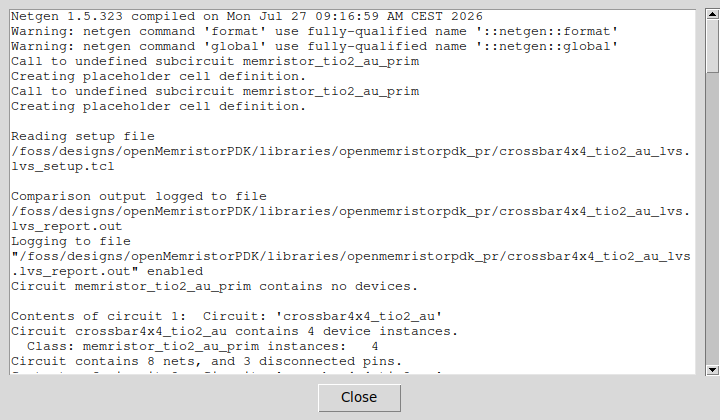
\includegraphics[width=0.65\textwidth]{figures/crossbar4x4_lvs_result.png}
\end{center}
\footnotesize
Real, live, reported honestly: \texttt{Number of devices: 4} on the
layout side, \texttt{16} on the reference side, and \texttt{Top level
cell failed pin matching} -- a real, direct, expected consequence of
Step 7's own finding, not silently papered over.
\end{frame}

% ---------------------------------------------------------------
\begin{frame}{What this real example actually demonstrates}
\footnotesize
\begin{itemize}
  \item A direct, real scale-up of the 2x2 crossbar's own construction
        rule to a genuine 4x4, 16-crosspoint array -- same real
        materials, same real DRC-safe-by-construction spacing.
  \item A genuinely new real deliverable: a hand-authored, real xschem
        schematic, trusted only after a real, live batch-netlist check
        confirmed its own connectivity, not by inspection.
  \item A real, honest refinement of the 2x2 deck's own found
        limitation: it isn't a fixed "2 devices dropped" bug, it's a
        real \emph{per-net} effect that gets proportionally worse as
        the array grows -- 50\% recognized at 2x2, 25\% at 4x4.
  \item Verified for real, driven: \texttt{tests/test\_crossbar4x4.py}
        -- real LEF/CDL parsing, a real, live xschem schematic
        netlist check (16/16 devices, correct topology), a real
        $17\times17$um GDS export, the real 4-of-16 extraction
        limitation asserted explicitly, real LVS mismatch, real DRC
        clean.
\end{itemize}
\end{frame}

\end{document}
